\documentclass[compress]{beamer}
%
% Choose how your presentation looks.
%
% For more themes, color themes and font themes, see:
% http://deic.uab.es/~iblanes/beamer_gallery/index_by_theme.html
%
\mode<presentation>
{
	\usetheme{Dresden}      % or try Darmstadt, Madrid, Warsaw, ...  
	%\useoutertheme{infolines} % split, tree, infolines
	%\useinnertheme{rectangles}
	\usecolortheme{orchid} % or try albatross, beaver, crane, ...
	\usefonttheme{structuresmallcapsserif}  % or try serif, structurebold, ...
	\setbeamertemplate{navigation symbols}{}
	\setbeamertemplate{caption}[numbered]
	\setbeamertemplate{footline}[frame number]
} 

\usepackage[english]{babel}
\usepackage[utf8x]{inputenc}
\usepackage{tikz}
\usetikzlibrary{trees,snakes,arrows}
\usepackage{tabularx}
\usepackage{subfig}
\usepackage{graphicx}
%\usepackage{animate}

\def\tobar{\mathrel{\mkern3mu  \vcenter{\hbox{$\scriptscriptstyle+$}}%
		\mkern-12mu{\to}}}

\title[BA Hobbhahn 2018]{Inverse Classification using Generative Models}
\author{Marius Hobbhahn}
\date{\today}

\begin{document}
	
	\begin{frame}
		\titlepage
	\end{frame}
	%
	% Uncomment these lines for an automatically generated outline.
	%\begin{frame}{Outline}
	%  \tableofcontents
	%\end{frame}
	%
	\section{Introduction}
	\subsection{ } % for the dots - there most probably is a more elegant solution.
	%
	\begin{frame}{Learning concepts more effectively}
		\begin{figure}
			\centering
			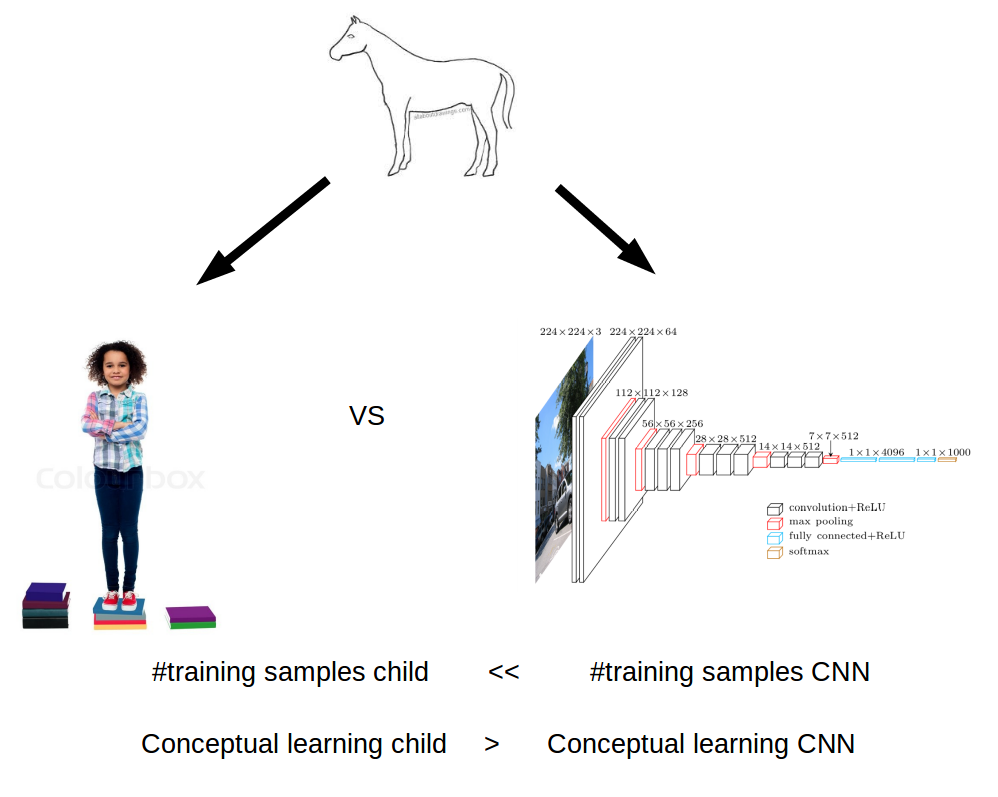
\includegraphics[width=0.8\textwidth]{images/intro_BA.png}
		\end{figure}
	\end{frame}
	%
	\begin{frame}{Sizes of popular datasets}
		\begin{itemize}
			\item Imagenet: 14,197,122 images
			\item MNIST: 70,000 images
			\item COCO: 330,000 images
			\item Twitter sentiment analysis: 1,578,627 tweets
			\item $\vdots$
		\end{itemize}
	\end{frame}
	%
	\section{Theory}
	\subsection{ } % for the dots - there most probably is a more elegant solution.
	\begin{frame}{Generative Model}
		\begin{figure}
			\centering
			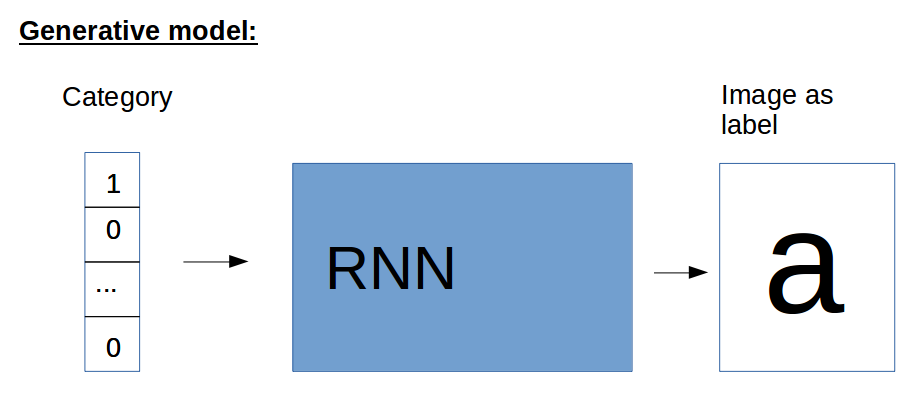
\includegraphics[width=0.8\textwidth]{images/generative_model.png}
		\end{figure}
	\end{frame}
	\begin{frame}{Inverse Classification}
		\begin{figure}
			\centering
			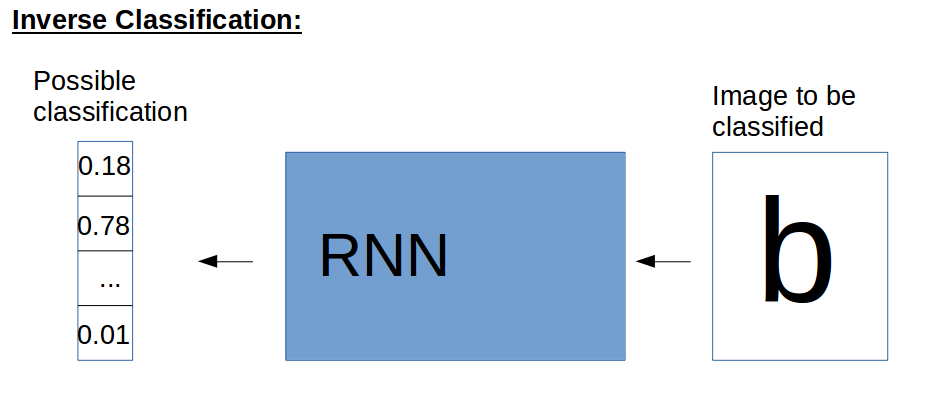
\includegraphics[width=0.8\textwidth]{images/inverse_classification.png}
		\end{figure}
	\end{frame}
	\begin{frame}{Structure}
		\begin{figure}
			\centering
			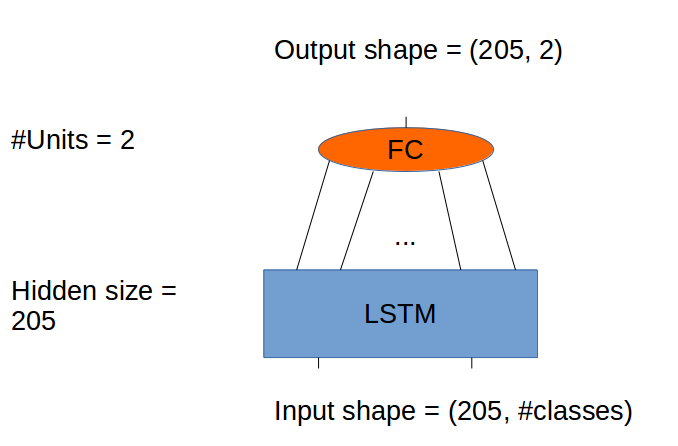
\includegraphics[width=0.8\textwidth]{images/generative_model_details.png}
		\end{figure}
	\end{frame}
	\section{Metrics}
	\subsection{ } % for the dots - there most probably is a more elegant solution.
	\begin{frame}{Heat Maps}
		\begin{figure}
			\centering
			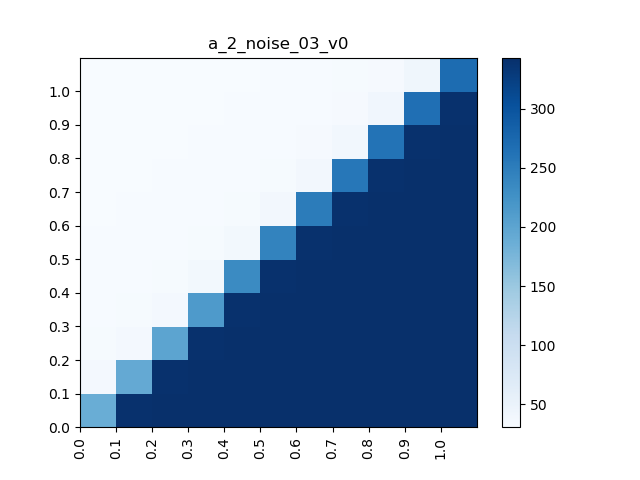
\includegraphics[width=0.8\textwidth]{images/a_2_noise_03_v0.png}
		\end{figure}	
	\end{frame}
	%
	\begin{frame}{Self-organizing feature Maps (SOMs)}
		\begin{figure}
			\centering
			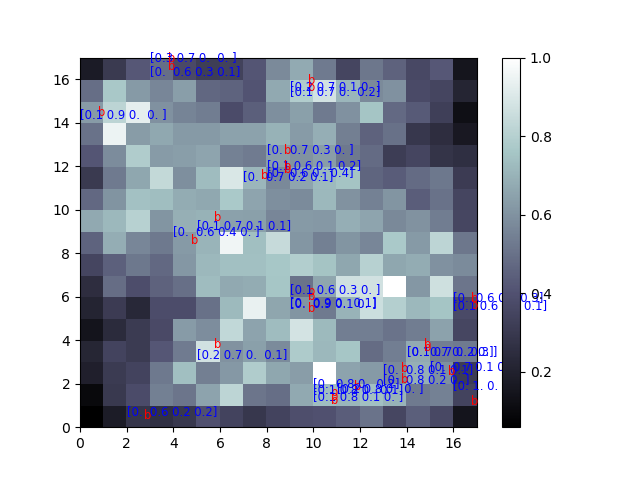
\includegraphics[width=0.8\textwidth]{images/17x17_4d_noise_01_v0_b.png}
			\caption{\textcolor{red}{character} 'b' and corresponding \textcolor{blue}{input vector}; color of background denotes average distance to neighboring nodes}
		\end{figure}
	\end{frame}
	%
	\begin{frame}{Accuracy and RMSE}
		\begin{table}[!htb]
			\centering
			\caption{Results for the 2D models without additions. The first five rows represent the accuracy and RMSE for each instance of the model while the last two show mean and standard deviation for each respective category.}
			\begin{tabularx}{\textwidth}{ X  X  X }
				\hline
				model & accuracy & RMSE \\ 
				\hline
				2\_naked\_v0 & 0.7 & 0.36\\
				2\_naked\_v1 & 0.57 & 0.44\\
				2\_naked\_v2 & 0.81 & 0.32 \\
				2\_naked\_v3 & 0.84 & 0.17 \\
				2\_naked\_v4 & 0.38 & 0.6 \\ 
				\hline
				mean & 0.66 & 0.38 \\
				standard deviation & 0.17 & 0.14 \\
				\hline
			\end{tabularx}
			\label{table:2_naked}
		\end{table}
	\end{frame}
	\section{Experiments}
	\subsection{ } % for the dots - there most probably is a more elegant solution.
	\begin{frame}{Model without additions}
		\begin{itemize}
			\item Train a simple generative model
			\item Investigate latent space 
			\item Test Inverse Classification
			\item (Additional experiment: add a second stack of LSTMs)
		\end{itemize}
	\end{frame}
	%
	\begin{frame}{Addition of Noise}
		\begin{itemize}
			\item Add a Gaussian noise layer and a clip layer to the model
			\item Train with standard deviation of 0.1, 0.2, 0.3 and 0.4
			\item proceed as before
			\item example: [0.93, 0.2, 0.13, 0.05]
		\end{itemize}
	\end{frame}
	%
	\begin{frame}{Repeller vector}
		\begin{itemize}
			\item Add a new class of uniformly distributed vectors with zero-sequences as targets of size $\frac{1}{\text{\#classes}}$ 
			\item proceed as before
			\item example: [0.25, 0.25, 0.25, 0.25]
		\end{itemize}
	\end{frame}
	%
	\begin{frame}{Addition of Types}
		\begin{itemize}
			\item Determine type of sequence through k-means clustering
			\item Give every input its type. It now becomes a 2D one-hot vector
			\item Test inverse classification and reduce type dimension with sum to become 1D one-hot vectors
			\item (Additional experiment: test with addition of noise)
			\item example: [[1,0,0,0], [0,0,0,0], [0,0,0,0], [0,0,0,0]]
		\end{itemize}
	\end{frame}
	%
	\begin{frame}{Sparse data}
		\begin{itemize}
			\item Take only the center of type clusters and train on them
			\item proceed as before
			\item (Additional experiment: test with addition of noise)
		\end{itemize}
	\end{frame}
	%
	\section{Results}
	\subsection{ } % for the dots - there most probably is a more elegant solution.
	%
	\begin{frame}{2D Latent Space (selected)}
		\begin{figure}
		\centering
		\begin{tabular}{cccc}
			\subfloat[]{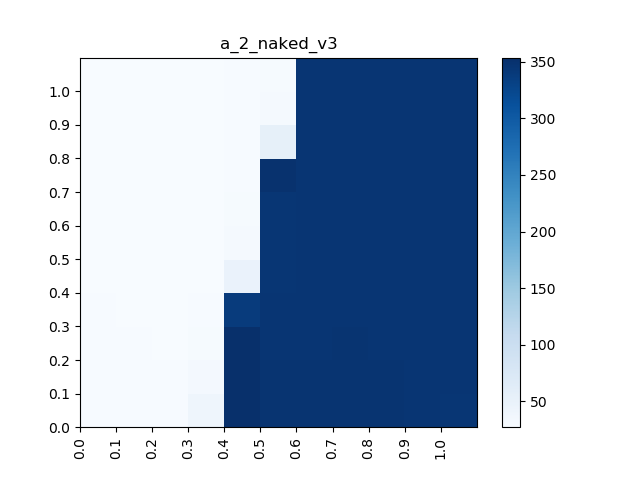
\includegraphics[width=2cm]{images/a_2_naked_v3.png}} 
			& \subfloat[]{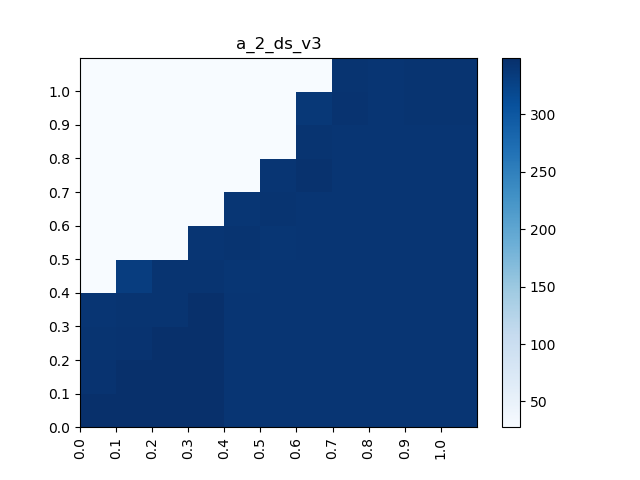
\includegraphics[width=2cm]{images/a_2_ds_v3.png}}
			& \subfloat[]{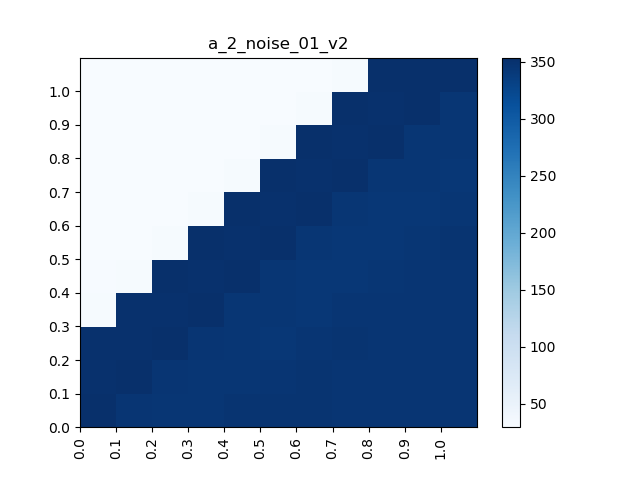
\includegraphics[width=2cm]{images/a_2_noise_01_v2.png}} 
			& \subfloat[]{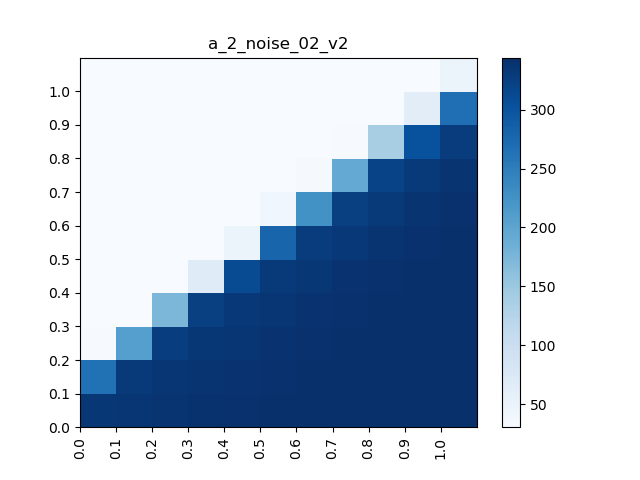
\includegraphics[width=2cm]{images/a_2_noise_02_v2.png}}
			\\
			\subfloat[]{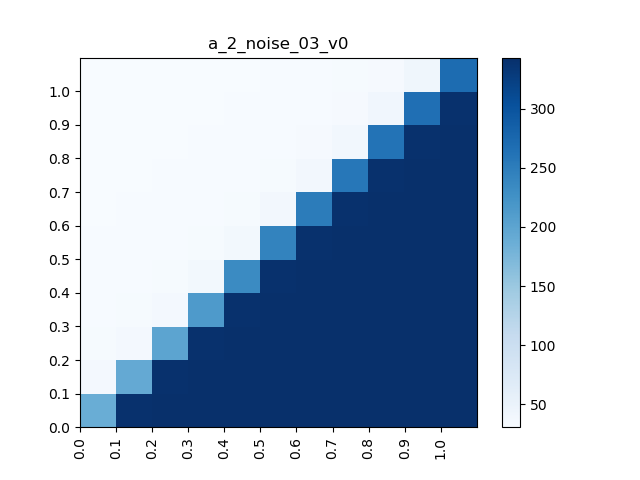
\includegraphics[width=2cm]{images/a_2_noise_03_v0.png}} 
			& \subfloat[]{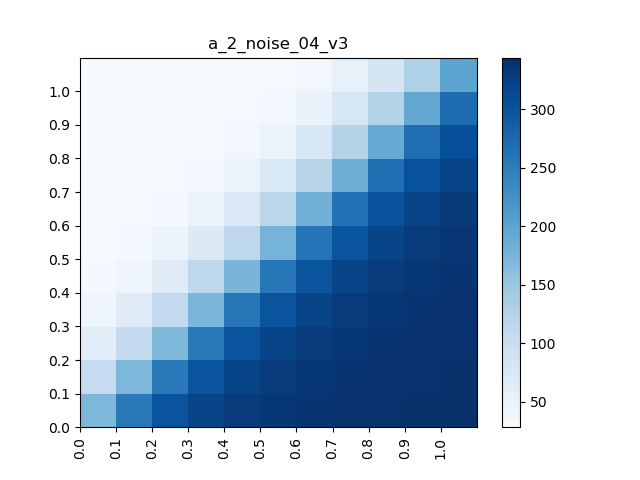
\includegraphics[width=2cm]{images/a_2_noise_04_v3.png}}
			& \subfloat[]{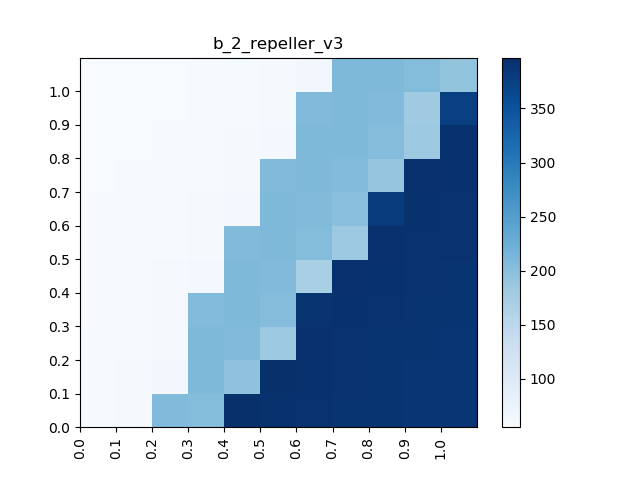
\includegraphics[width=2cm]{images/b_2_repeller_v3.png}}
			& \subfloat[]{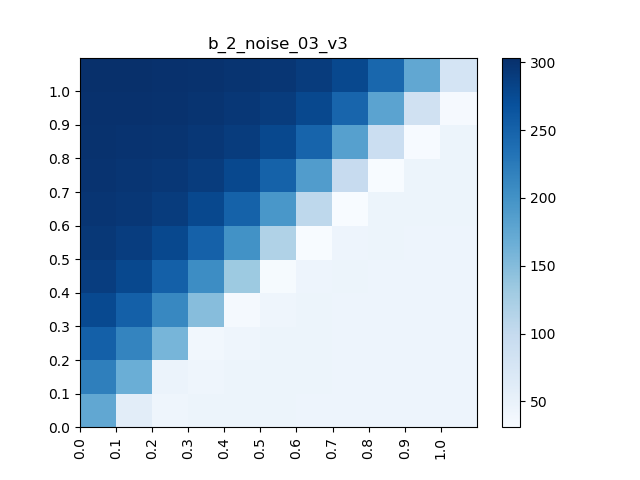
\includegraphics[width=2cm]{images/b_2_noise_03_v3.png}}
		\end{tabular}
		\caption{(A) Naked; (B) double-stacked; (C) Noise\_01; (D) Noise\_02; (E) Noise\_03; (F) Noise\_04; (G) Repeller; (H) Noise\_03\_B}
		\end{figure}
	\end{frame}
	%
%	\begin{frame}{4D Latent space (selected)}
%		Trends within SOMs
%		\begin{itemize}
%			\item Vectors with similar properties tend to cluster at neurons with small distances
%			\item Borders between different character classes are visible
%			\item Addition of noise: borders become more fuzzy but do not overlap
%		\end{itemize}
%	\end{frame}
	%
	\begin{frame}{2D}
		\begin{table}[!htb]
			\centering
			\begin{tabularx}{\textwidth}{p{5cm} X}
				\hline
				model & accuracy \\ 
				\hline
				naked\_2 & 0.66 \\
				ds\_2 & \textcolor{red}{0.54} \\
				noise\_01\_2 & \textcolor{green}{0.67} \\
				noise\_02\_2 & \textcolor{blue}{0.98} \\
				noise\_03\_2 & \textcolor{blue}{1.0} \\
				noise\_04\_2 & \textcolor{blue}{1.0} \\
				repeller\_2 & \textcolor{green}{0.79} \\
				types\_2 & \textcolor{green}{0.79} \\
				types\_noise\_04\_2 & \textcolor{green}{0.85} \\
				sparse\_noise\_04\_2 & \textcolor{blue}{0.97} \\
				comparison\_mse\_2 & \textcolor{blue}{1.0} \\
				comparison\_sparse\_2 & \textcolor{blue}{0.98} \\
				random\_values & 0.5 \\
				\hline
				\end{tabularx}
			\label{table:comparison_all}
		\end{table}
	\end{frame}
	%
	\begin{frame}{4D}
		\begin{table}[!htb]
			\centering
			\begin{tabularx}{\textwidth}{p{5cm} X }
				\hline
				model & accuracy \\ 
				\hline
				naked\_4 & 0.49 \\
				ds\_4 & \textcolor{green}{0.65} \\
				noise\_01\_4 & \textcolor{green}{0.88} \\
				noise\_02\_4 & \textcolor{blue}{0.91} \\
				noise\_03\_4 & \textcolor{blue}{0.93} \\
				noise\_04\_4 & \textcolor{blue}{0.93} \\
				repeller\_4 & \textcolor{green}{0.58} \\
				types\_4 & \textcolor{red}{0.27} \\
				types\_noise\_04\_4 & \textcolor{green}{0.79} \\
				sparse\_noise\_04\_4 & \textcolor{blue}{0.97} \\
				comparison\_mse\_4 & \textcolor{blue}{0.94} \\
				comparison\_sparse\_4 & \textcolor{blue}{0.94} \\		
				random\_values & 0.25 \\
				\hline
			\end{tabularx}
			\label{table:comparison_all_4}
		\end{table}
	\end{frame}
	%
	\begin{frame}{20D}
		\begin{table}[!htb]
			\centering
			\begin{tabularx}{\textwidth}{p{5cm} X }
				\hline
				model & accuracy \\ 
				\hline
				naked\_20 & 0.35 \\
				ds\_20 & \textcolor{red}{0.32} \\
				noise\_01\_20 & 0.35 \\
				noise\_02\_20 & \textcolor{green}{0.38} \\
				noise\_03\_20 & \textcolor{green}{0.43} \\
				noise\_04\_20 & \textcolor{red}{0.2} \\
				repeller\_20 & \textcolor{red}{0.29} \\
				types\_20 & \textcolor{red}{0.08} \\
				types\_noise\_03\_20 & \textcolor{red}{0.09} \\
				sparse\_noise\_03\_20 & \textcolor{green}{0.49} \\
				comparison\_mse\_20 & \textcolor{blue}{0.97} \\
				comparison\_sparse\_20 & \textcolor{green}{0.61} \\
				random\_values & 0.05 \\
				\hline
			\end{tabularx}
			\label{table:comparison_all_20}
		\end{table}
	\end{frame}
	\section{Conclusion}
	\subsection{ } % for the dots - there most probably is a more elegant solution.
	\begin{frame}{Results as plot}
		\begin{figure}
			\centering
			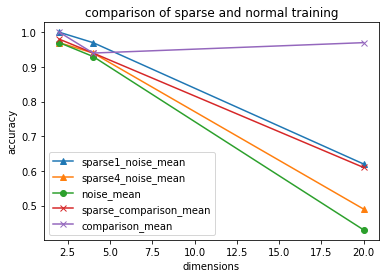
\includegraphics[width=0.8\textwidth]{images/result_plot.png}
		\end{figure}
	\end{frame}
	\begin{frame}{Conclusions}
	\begin{block}{Conclusion 1}
		The Inverse Classification is as good as the conceptual representation of the latent space.
	\end{block}
	\hspace{2cm}
	\begin{block}{Conclusion 2}
		The Inverse Classification is (at least for this task) invariant to the number of training data.
	\end{block}
	\end{frame}
	\section{Further Investigation and Appendix}
	\subsection{ } % for the dots - there most probably is a more elegant solution.
	\begin{frame}{Sparse\_1\_noise\_04}
		\begin{table}[!htb]
			\centering
			\caption{Sparse\_1\_noise\_04 average accuracy and RMSE}
			\begin{tabularx}{\textwidth}{ p{5cm}  X  X }
				\hline
				model & accuracy & RMSE \\ 
				\hline
				2\_sparse\_1\_noise\_04 & 1.0 & 0.13\\
				4\_sparse\_1\_noise\_04 & 0.97 & 0.18\\
				20\_sparse\_1\_noise\_03\_v2 & 0.62 & 0.18\\
				\hline
			\end{tabularx}
			\label{table:sparse1_noise_04}
		\end{table}
	\end{frame}
	%
	\begin{frame}{SOM trends 1}
		\begin{itemize}
			\item Vectors with similar properties tend to cluster at neurons with small distances. 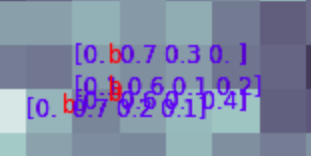
\includegraphics[width=0.5\textwidth]{images/SOM_similar_vector_cluster.png}
		\end{itemize}
	\end{frame}
	%
	\begin{frame}{SOM trends 2}
		\begin{itemize}
			\item Borders between classes are visible \\
			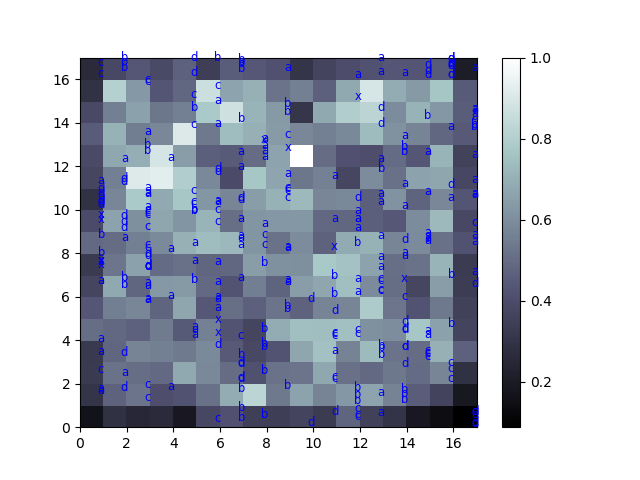
\includegraphics[width=0.7\textwidth]{images/SOM_naked.png}
		\end{itemize}
	\end{frame}
	%
	\begin{frame}{SOM trends 3}
		\begin{itemize}
			\item Addition of noise: borders become more fuzzy but do not overlap \\
			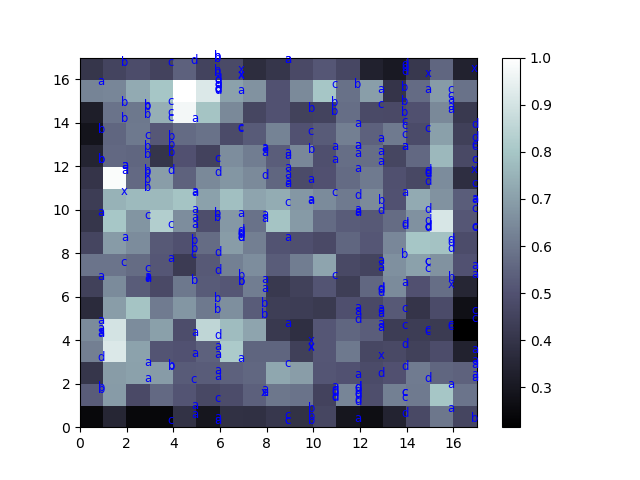
\includegraphics[width=0.7\textwidth]{images/SOM_noise.png}
		\end{itemize}
	\end{frame}	
	%\begin{frame}{Embedded Animation}
	%	%\animategraphics[loop,controls,width=\linewidth]{10}{4_noise_04_v0-}{0}{285}
	%\end{frame}
\end{document}
